\section{Inelastic scattering into collective modes}\label{sec:17.3}

A dark-matter particle of \SI{10}{keV} at the largest laboratory speed $v_{\mathrm{max}}$ carries \SI{35}{meV} of kinetic energy, just short of the \SI{36.35}{meV} longitudinal optical phonon of GaAs, and elastic scattering cannot create that phonon below \SI{10.35}{keV} (\cref{sec:11.2}). Let the same particle arrive in an excited state \SI{1}{eV} above its ground state and leave in the lower one. It then emits the phonon at every speed of the halo, at a rate of $2.6\times10^4$ events per kilogram and year for a light dark photon at $\sigmae = \SI{e-40}{cm^2}$. \Cref{sec:10.9} followed the splitting $\Delta_\chi$ through the electron-recoil spectrum of silicon. The collective modes, phonons, magnons and plasmons, are the natural final states of down-scattering (\cref{sec:8.2-exothermic}): the band of allowed $(\vect{q},\omega)$ moves up by $|\Delta_\chi|$, and a mode whose energy lies below the splitting is always reached. One formula covers all the modes, and the dispersion of each mode decides where its line lies, how wide it is, and how much of the splitting it takes.

\subsection{Down-scattering into a collective mode}\label{sec:17.3-shell}

Every collective response of \cref{chap:10,chap:11,chap:14} is, at $T = 0$, a sum of lines. The one-phonon response \cref{eq:11.1-S1}, the one-magnon response \cref{eq:14.1-Safm} and the plasmon pole of \cref{eq:4.5-plasmonL} each put a weight on the dispersion surface $\omega = \omega_\nu(\vect{q})$ of a branch $\nu$. Contracted with the dark-matter tensor, the integrand of \cref{eq:8.2-spectrum} becomes
\begin{equation}
  \sum_{ab}\mathfrak{D}_{ab}(\vect{q})\,S_{ab}(\vect{q},\omega) = \frac{2\pi}{\Omega}\sum_\nu\mathcal{Y}_\nu(\vect{q})\,\delta\bigl(\omega - \omega_\nu(\vect{q})\bigr) ,
  \label{eq:17.3-lines}
\end{equation}
which defines the mode weight $\mathcal{Y}_\nu \ge 0$. For the nucleon coupling of \cref{sec:11.1}, in the notation of \cref{eq:11.1-S1} (nucleon numbers $A_\kappa$, polarization vectors $\vect{e}_{\kappa\nu}$), $\mathcal{Y}_\nu = |\tilde V_N|^2|\sum_\kappa A_\kappa\ee^{-W_\kappa}\ee^{\ii\vect{q}\cdot\vect{\tau}_\kappa}\vect{q}\cdot\vect{e}^*_{\kappa\nu}/\sqrt{M_\kappa}|^2/2\omega_\nu$. For the spin coupling $\mathcal{O}_4$ in an antiferromagnet, with $\Omega = \Omega_{\mathrm{ion}}$, the contraction \cref{eq:14.1-contract} gives $\mathcal{Y} = \tfrac14|\vect{S}||c_4|^2|F^{\mathrm{mag}}|^2w^{\mathrm{M}}_{\vect{q}}$, with the coupling $c_4$, the magnetic form factor $F^{\mathrm{mag}}$ and the magnon weight $w^{\mathrm{M}}_{\vect{q}}$ of \cref{sec:14.1}. For the plasmon of an electron gas coupled through the electron density, $S = (2q^2/e^2)L$ and the pole carries the weight $\pi/(\partial\varepsilon_1/\partial\omega)$, so that $\mathcal{Y} = \Omega|\tilde V|^2q^2/[e^2\,\partial\varepsilon_1/\partial\omega]$.

Down-scattering has $\Delta_\chi < 0$, and energy conservation, $\omega_{\vect{q}} = \omega_\nu(\vect{q})$ with $\omega_{\vect{q}}$ of \cref{eq:1.3-omegaq}, reads
\begin{equation*}
  |\Delta_\chi| + \vect{q}\cdot\vect{v} - \frac{q^2}{2\mchi} = \omega_\nu(\vect{q}) .
\end{equation*}
We first set $\vect{v} = 0$. Along each direction $\hat{\vect{q}}$ the condition fixes the magnitude of the momentum transfer at the roots $q_\nu(\hat{\vect{q}})$ of
\begin{equation}
  |\Delta_\chi| - \frac{q_\nu^2}{2\mchi} = \omega_\nu(q_\nu\hat{\vect{q}}) ,
  \label{eq:17.3-qnu}
\end{equation}
and we write $v_\nu = q_\nu/\mchi$ for the speed of the outgoing particle relative to the incoming one. For a mode whose energy is small against the splitting, $q_\nu \simeq (2\mchi|\Delta_\chi|)^{1/2}$; at a fixed deposit $\omega$ this is the shell momentum $q_\Delta$ of \cref{sec:10.9}. As a function of $q$ along $\hat{\vect{q}}$, the argument of the delta function has the slope $-(q/\mchi + u_\nu)$, with $u_\nu = \hat{\vect{q}}\cdot\nabla_{\vect{q}}\,\omega_\nu$ the group velocity of the mode along $\vect{q}$. Writing $\dd^3q = q^2\dd q\,\dd^2\hat{\vect{q}}$, the radial integral picks up $q_\nu^2/(q_\nu/\mchi + u_\nu)$ at each root. The rate of one particle, $\varGamma = \int\dd\omega\int\dd^3q/(2\pi)^3\,\sum\mathfrak{D}_{ab}S_{ab}\,\delta(\omega - \omega_{\vect{q}})$, is then $(2\pi)^{-3}(2\pi/\Omega)\sum_\nu\int\dd^2\hat{\vect{q}}\,q_\nu^2\mathcal{Y}_\nu/(q_\nu/\mchi + u_\nu)$, which summed over branches and directions reads
\begin{keyresult}[Exothermic rate into a collective mode]
\begin{equation}
  \varGamma = \frac{\mchi}{\pi\Omega}\sum_\nu\Bigl\langle\frac{q_\nu\,\mathcal{Y}_\nu(q_\nu\hat{\vect{q}})}{1 + u_\nu/v_\nu}\Bigr\rangle_{\hat{\vect{q}}}\Bigl[1 + O\bigl(v^2/v_\nu^2\bigr)\Bigr] , \qquad
  \mathcal{R} = \frac{\rho_\chi}{\mchi\rho_T}\,\varGamma ,
  \label{eq:17.3-rate}
\end{equation}
with $q_\nu$ the roots of \cref{eq:17.3-qnu}, $\langle\cdot\rangle_{\hat{\vect{q}}}$ the average over directions, and $\mathcal{R}$ the rate per unit target mass. It holds for $v_\nu$ above the speeds of the halo and for a weight $\mathcal{Y}_\nu$ that varies little over momenta $\mchi v_{\mathrm{max}}$.
\end{keyresult}
\noindent At finite $\vect{v}$ the surface of \cref{eq:17.3-qnu} moves by a vector of order $\mchi\vect{v}$ and changes its radius at second order. The term linear in $\vect{v}$ averages to zero over a weight and a dispersion even in $\vect{q}$, as for the electronic shell of \cref{eq:10.9-shell}, and the correction to the rate is of order $v^2/v_\nu^2$. The deposited energy, by contrast, shifts at first order, and \cref{sec:17.3-lines} shows that this sets the width of the line. The factor $(1 + u_\nu/v_\nu)^{-1}$ is new compared with the electronic shell, where the energy is integrated at fixed $\omega$. It is close to one for phonons and magnons, whose group velocities, $10^{-5}$ to $10^{-4}$, lie far below $v_\nu$, but not for the plasmon, whose dispersion is steep.

The velocity independence has a simple reading in the incoherent limit. For a free scatterer the rate per particle of elastic scattering is $\nd\sigma v$, and that of exothermic down-scattering is $\nd\sigma v_\nu$: the final momentum, and with it the phase space, is fixed by the splitting rather than by the incoming speed. The magnons of NiO show it. With the spin coupling $\mathcal{O}_4$, a heavy mediator and $\sigmae = \SI{e-40}{cm^2}$ (the setting of \cref{fig:14-nio-rate}), a particle of \SI{1}{MeV} with $|\Delta_\chi| = \SI{10}{eV}$ has $q_\nu = \SI{4.45}{keV}$, beyond the ordering wavevector at \SI{2.58}{keV}. The shell then crosses many magnetic zones, and the direction average of the weight is 1.149, close to its zone average 1.156 (in the spin-wave theory of \cref{we:14-nio}, $1 + 2\Delta S = 1.157$, with $\Delta S$ the zero-point spin reduction). \Cref{eq:17.3-rate} yields 8210 events per kilogram and year, within \SI{3}{\percent} of the full integral over the halo, 8000, against 2620 for elastic scattering at the same mass.

\subsection{Line positions and widths}\label{sec:17.3-lines}

Each root of \cref{eq:17.3-qnu} deposits $\omega_\nu(q_\nu\hat{\vect{q}})$. The splitting is shared between the outgoing dark matter, which keeps $q_\nu^2/2\mchi$, and the mode, and the dispersion decides the share. A parabolic branch, $\omega_\nu(\vect{q}) = \omega_\nu(0) + q^2/2m^*_\nu$ with a dispersion mass $m^*_\nu$ of either sign, makes this exact for any $\vect{v}$. Energy conservation becomes $|\Delta_\chi| - \omega_\nu(0) + \vect{q}\cdot\vect{v} = q^2/2\mu_\nu$ with $\mu_\nu = \mchi m^*_\nu/(\mchi + m^*_\nu)$, and completing the square,
\begin{gather}
  |\vect{q} - \mu_\nu\vect{v}|^2 = q_\nu^2 + \mu_\nu^2v^2 , \qquad
  q_\nu^2 = 2\mu_\nu\bigl(|\Delta_\chi| - \omega_\nu(0)\bigr) , \notag\\
  \omega_\nu(q_\nu) = \omega_\nu(0) + \frac{\mu_\nu}{m^*_\nu}\bigl(|\Delta_\chi| - \omega_\nu(0)\bigr) .
  \label{eq:17.3-parabolic}
\end{gather}
The momentum transfers lie on a sphere centered at $\mu_\nu\vect{v}$, and at $\vect{v} = 0$ the mode takes the fraction $\mu_\nu/m^*_\nu = \mchi/(\mchi + m^*_\nu)$ of the energy above its bottom. A free electron at rest is the branch $\omega(0) = 0$, $m^* = m_e$, and \cref{eq:17.3-parabolic} returns the line $(\mu_{\chi e}/m_e)|\Delta_\chi|$ of \cref{sec:10.9-inelastic}. A flat branch, $|m^*_\nu| \gg \mchi$, takes little more than $\omega_\nu(0)$ and leaves the rest of the splitting to the dark matter. A steep branch, $m^*_\nu \ll \mchi$, takes nearly all of it.

The width follows from the same sphere. On it $q^2 = q_\nu^2 + 2\mu_\nu^2v^2 + 2\mu_\nu\vect{v}\cdot(\vect{q} - \mu_\nu\vect{v})$, and the deposited energy $\omega_\nu(0) + q^2/2m^*_\nu$ differs from the line $\omega_\nu(q_\nu)$ by $(\mu_\nu q_\nu v/m^*_\nu)\cos\theta$ plus a shift of order $v^2$, with $\theta$ the angle between $\vect{v}$ and $\vect{q} - \mu_\nu\vect{v}$. For a weight that is the same in every direction, $\cos\theta$ is uniform on the sphere, and a particle of speed $v$ spreads its energy uniformly over a band of full width $2\mu_\nu q_\nu v/|m^*_\nu|$. Averaging over the halo with the factor $1/v$ of this normalization turns the band into $\eta$:
\begin{equation}
  \frac{1}{\varGamma_\nu}\frac{\dd\varGamma_\nu}{\dd\omega} = \frac{|m^*_\nu|}{2\mu_\nu q_\nu}\;\eta\Bigl(\frac{|m^*_\nu|\,|\omega - \omega_\nu(q_\nu)|}{\mu_\nu q_\nu}\Bigr) ,
  \label{eq:17.3-profile}
\end{equation}
to first order in $v/v_\nu$, normalized by $\int_0^\infty\eta(u)\,\dd u = 1$. The line has the shape of $\eta(\vmin)$ reflected about its center. It is flat near the center, where every particle contributes, falls to half height where $\eta$ does, at \SI{278}{km/s} or 0.35 of $v_{\mathrm{max}}$, and ends at the full width $2\mu_\nu q_\nu v_{\mathrm{max}}/|m^*_\nu|$. For a branch that is not parabolic, the same steps with the dispersion linearized about $q_\nu$ replace $q_\nu/m^*_\nu$ by $u_\nu$ and $\mu_\nu$ by $\mchi$, as long as $|u_\nu| \ll v_\nu$: the full width is $2|u_\nu|\mchi v_{\mathrm{max}}$. Intrinsic widths of the mode, from anharmonic decay of a phonon or Landau and interband damping of a plasmon, add by convolution.

An acoustic branch, $\omega = c_\nu q$, has $q_\nu = \mchi[(c_\nu^2 + 2|\Delta_\chi|/\mchi)^{1/2} - c_\nu]$ and a line at $c_\nu q_\nu$ whose full width relative to its energy is $2v_{\mathrm{max}}/v_\nu$. It is a line as long as $v_\nu$ is well above $v_{\mathrm{max}}$ and $q_\nu$ still lies inside the zone. Antiferromagnetic magnons near $\Gamma$ behave the same way. In NiO at \SI{0.1}{MeV} and $|\Delta_\chi| = \SI{1}{eV}$, $q_\nu = \SI{435}{eV}$, and the magnons emitted at $\vect{v} = 0$ have \SI{55.1}{meV} with a spread of \SI{0.9}{meV} over directions. However, $v_{\mathrm{max}}/v_\nu = 0.61$, and with the mean group velocity $1.1\times10^{-4}$ the halo spreads them over a full width $2|u_\nu|\mchi v_{\mathrm{max}} = \SI{60}{meV}$, more than the line energy. Their weight there, 0.28 on average, includes the suppression near $\Gamma$ of \cref{sec:14.1}, and \cref{eq:17.3-rate} yields 5130 events per kilogram and year against 5710 from the full integral and 434 for elastic scattering. Once $q_\nu$ crosses many zones, the deposited energies sample the whole branch, and the spectrum becomes the weighted density of states: \SI{100}{meV} on average, with a spread of \SI{15}{meV}, for NiO at \SI{1}{MeV} and $|\Delta_\chi| = \SI{10}{eV}$.

The magnons of a ferromagnet start at the Larmor frequency and disperse quadratically near $\Gamma$, a parabolic branch with $\omega_\nu(0) = \omega_{\mathrm{Lar}}$ and a positive $m^*_\nu$. As $|\Delta_\chi|$ approaches $\omega_{\mathrm{Lar}}$, $q_\nu \to 0$ and \cref{eq:17.3-rate} vanishes in proportion to $q_\nu$ for a coupling without $q$ dependence. The uniform precession of \cref{sec:14.3} is the end point of the exothermic spectrum, where the halo speeds take over from the splitting.

A flat optical branch gives a narrow line at its own energy, and \cref{we:17-gaas} works it out for GaAs.

The plasmon is the steep case. Expanding the gas dispersion of \cref{sec:4.5}, $\omega_{\mathrm{pl}} \simeq \omega_p + \alpha_{\mathrm{pl}}q^2/m_e$, gives $m^*_{\mathrm{pl}} = m_e/2\alpha_{\mathrm{pl}}$. At the valence density of silicon, $E_{\mathrm{F}} = \SI{12.47}{eV}$, $\omega_p = \SI{16.61}{eV}$ and $\alpha_{\mathrm{pl}} = \tfrac35E_{\mathrm{F}}/\omega_p = 0.451$, so that $m^*_{\mathrm{pl}} = \SI{567}{keV}$, lighter than the dark matter of most electron-recoil searches. A particle of \SI{1}{MeV} has $\mu_{\mathrm{pl}} = \SI{362}{keV}$ and hands the plasmon 0.638 of the splitting above $\omega_p$, a particle of \SI{10}{MeV} 0.946. At $|\Delta_\chi| = \SI{20}{eV}$ and \SI{1}{MeV}, \cref{eq:17.3-parabolic} puts the line at \SI{18.77}{eV} and $q_\nu = \SI{1.57}{keV}$, and the exact zero of the Lindhard function at \SI{18.83}{eV} and \SI{1.53}{keV}. The steep dispersion that hands the plasmon the splitting also makes the line wide: the full width from the halo is \SI{5.3}{eV}, more than the measured \SI{3.66}{eV} width of the silicon loss peak (\cref{sec:4.5}). Since the plasmon exists only below the Landau-damping momentum, the line exists only in a window of splittings. The parabolic dispersion meets the upper edge of the pair continuum, $qv_{\mathrm{F}} + q^2/2m_e$, at \SI{2.30}{keV}, and the window closes \SI{7.3}{eV} above $\omega_p$ at \SI{1}{MeV}.

\begin{workedexample}{Exothermic emission of an optical phonon in GaAs}\label{we:17-gaas}
Take a dark photon, $\sigmae = \SI{e-40}{cm^2}$ as in \cref{sec:11.2}, $\mchi = \SI{30}{keV}$ and $\Delta_\chi = \SI{-1}{eV}$. The splitting lies below the gap of GaAs, \SI{1.52}{eV}, so no electronic excitation is open, and the dark photon reaches the lattice through the longitudinal optical phonon alone. Its line in the loss function carries $(\pi\omega_{\mathrm{L}}/2)(1 - \omega_{\mathrm{T}}^2/\omega_{\mathrm{L}}^2)/\varepsilon_\infty = \SI{7.59e-4}{eV}$ with the measured $\omega_{\mathrm{T}} = \SI{33.62}{meV}$, $\omega_{\mathrm{L}} = \SI{36.35}{meV}$ and $\varepsilon_\infty = 10.88$ (\cref{eq:11.2-onebranch}, splitting route). With this line in place of the averaged loss function $\bar L$ of \cref{eq:10.9-shell}, that equation times $(1 + u_\nu/v_\nu)^{-1}$ is \cref{eq:17.3-rate} for the charge coupling:
\begin{equation*}
  \mathcal{R} = \frac{\rho_\chi\,\sigmae\,q_\nu^3\,\FDM(q_\nu)^2\,\omega_{\mathrm{L}}}{2e^2\rho_T\,\mu_{\chi e}^2}\,\frac{1}{\varepsilon_\infty}\Bigl(1 - \frac{\omega_{\mathrm{T}}^2}{\omega_{\mathrm{L}}^2}\Bigr)\frac{1}{1 + u_\nu/v_\nu} .
\end{equation*}

\emph{Kinematics.} With the computed dispersion of the longitudinal branch of \cref{sec:5.5}, shifted to the measured $\omega_{\mathrm{L}}$ at $\Gamma$ and averaged over $[100]$, $[110]$ and $[111]$, \cref{eq:17.3-qnu} gives $q_\nu = \SI{240.5}{eV}$, 0.109 of $2\pi/a$ and inside the region where the Born-charge vertex holds (\cref{sec:11.2}). Then $v_\nu = 8.0\times10^{-3}$ and $v_{\mathrm{max}}/v_\nu = 0.33$. The estimate $2.5\langle v^2\rangle/v_\nu^2$ of \cref{sec:10.9} puts the halo correction to the rate at \SI{6}{\percent}.

\emph{Line.} The branch falls with $q$, $u_\nu = -6.2\times10^{-7}$, and the line lies at \SI{36.279}{meV}, \SI{0.071}{meV} below $\omega_{\mathrm{L}}$, between 36.256 and \SI{36.314}{meV} depending on the direction. Its full width from the halo, $2|u_\nu|\mchi v_{\mathrm{max}}$, is \SI{0.099}{meV}, and its half-maximum width 0.35 of that. Both are below the anharmonic width of the phonon, a fraction of a meV (\cref{sec:11.2}). The dark matter keeps \SI{0.964}{eV}; the detector sees one optical phonon.

\emph{Rate.} For a light dark photon, $\FDM = (q_0/q)^2$, the formula yields 1817 events per kilogram and year, and the full integral over the halo with the absolute value in $\vmin$ (\cref{eq:10.9-inel}) 1810. Elastic scattering at the same mass leads to 842, so the splitting doubles the rate while fixing the energy deposited. For a heavy dark photon the shell form is at 0.0314 and the full integral 0.0334, against $5.7\times10^{-5}$ for elastic scattering, a gain of 585. The two mediators respond oppositely to the splitting, since the light one weights $q_\nu^{-1}$ and the heavy one $q_\nu^3$. At $|\Delta_\chi| = \SI{0.5}{eV}$ the full integrals give 2600 for the light dark photon and 0.012 for the heavy one; the shell form yields 2620 and 0.010, off by \SI{12}{\percent} for the heavy mediator, which weights the largest momenta, at $v_{\mathrm{max}}/v_\nu = 0.48$.

\emph{Below the elastic edge.} At \SI{10}{keV}, under the edge $2\omega_{\mathrm{L}}/v_{\mathrm{max}}^2 = \SI{10.35}{keV}$, elastic scattering is closed. The same splitting gives $q_\nu = \SI{138.8}{eV}$, $v_{\mathrm{max}}/v_\nu = 0.19$, and $2.6\times10^4$ events per kilogram and year for the light dark photon, with the shell form within \SI{0.1}{\percent} of the full integral.
\end{workedexample}

\subsection{Electronic and collective channels in silicon}\label{sec:17.3-silicon}

\begin{figure}[tbp]
  \centering
  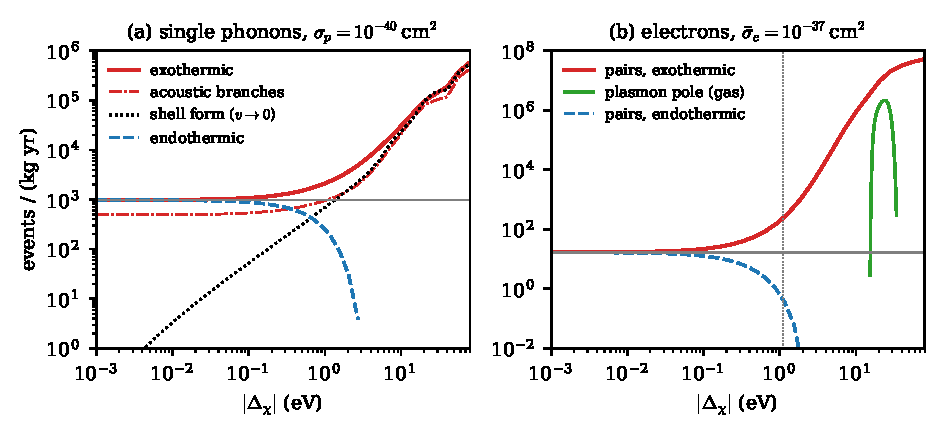
\includegraphics[width=\linewidth]{figures/ch17/fig17_3.pdf}
  \caption{Rates of silicon per kilogram and year against the mass splitting for $\mchi = \SI{1}{MeV}$, heavy mediator, standard halo of \cref{sec:1.2}, $T = 0$. Solid: exothermic ($\Delta_\chi = -|\Delta_\chi|$); dashed: endothermic ($\Delta_\chi = +|\Delta_\chi|$); gray line: elastic scattering. (a) Single phonons for a coupling to the nucleon number, $\sigma_p = \SI{e-40}{cm^2}$: the one-phonon response \cref{eq:11.1-S1} with all six branches of the computed phonons of \cref{sec:5.2} at the actual $\vect{q}$ (Umklapp and Debye--Waller factor included), averaged over the orientations of the crystal, deposits $\omega \ge \SI{1}{meV}$; dash-dotted: the three lowest branches; dotted: the shell form \cref{eq:17.3-rate}. (b) Electrons for a coupling to the electron density, $\sigmae = \SI{e-37}{cm^2}$: pairs from \cref{eq:10.9-inel} with the random-phase loss function with local fields of the tables of \cref{sec:10.2}, above \SI{1.11}{eV}, the step-model gap of their package (dotted vertical line; the tables are scissored to \SI{1.17}{eV}, \cref{sec:10.10}), the loss function held at its first tabulated momentum, \SI{493}{eV}, below it; green: the plasmon pole of an electron gas at the valence density of silicon, \cref{eq:10.3-plrate} with the splitting in $\vmin$, a model of the plasmon part of the electronic rate.}
  \label{fig:17-exo}
\end{figure}

\Cref{fig:17-exo} puts the two couplings of silicon side by side at \SI{1}{MeV}, each at its reference cross-section. Their elastic rates are 976 events per kilogram and year for single phonons and 16.7 for pairs. A particle of that mass carries up to $\tfrac12\mchi v_{\mathrm{max}}^2 = \SI{3.51}{eV}$, and a splitting well below this changes little: at $|\Delta_\chi| = \SI{0.12}{eV}$ the two rates are 1.12 and 1.39 times their elastic values. Above a few eV the splitting dominates, and the two channels respond to it differently.

The single-phonon rate rises from $2.0\times10^3$ at \SI{0.94}{eV} to $3.2\times10^4$ at \SI{10.3}{eV} and $5.8\times10^5$ at \SI{80}{eV}. The momentum transfer $q_\nu \simeq (2\mchi|\Delta_\chi|)^{1/2}$ grows from \SI{1.4}{keV} to \SI{12.6}{keV}, from $0.6$ to $5.6\,q_{\mathrm{BZ}}$. The one-phonon weight grows as $q^2$ times the Debye--Waller factor, whose exponent $2W$ is still just 0.10 at \SI{80}{eV}; two-phonon emission is smaller than one-phonon emission by a factor of order $W$. The deposited energy does not follow the splitting. Beyond the zone the shell crosses every branch, the spectrum is the weighted density of phonon states, and at \SI{10}{eV} the mean deposit is \SI{34.5}{meV}, with \SI{42}{\percent} above \SI{40}{meV} in the optical branches. A detector reading phonons sees the same energies as for elastic scattering, with a rate raised by a factor of 31 at \SI{10}{eV}. Between 10.3 and \SI{80}{eV} the shell form lies at 0.78 to 1.10 of the full integral. The residual comes from the condition on the weight in \cref{eq:17.3-rate}, not from the halo speeds, whose correction is $(v_{\mathrm{max}}/v_\nu)^2 \le 0.34$ there: the one-phonon weight varies on the scale $q_{\mathrm{BZ}} = \SI{2.25}{keV}$, smaller than $\mchi v_{\mathrm{max}} = \SI{2.65}{keV}$, and a single momentum per direction misses that structure.

The electronic rate rises far more steeply, from 165 at \SI{0.94}{eV} to $9.6\times10^5$ at \SI{10.3}{eV} and $5.3\times10^7$ at \SI{80}{eV}, a gain of $3\times10^6$ over the elastic rate. Elastic scattering at \SI{1}{MeV} barely crosses the gap, so any energy the splitting adds opens phase space that was nearly closed. Here the deposit does follow the splitting: \cref{sec:10.9} found the spectrum peaked between the gap and the plasma frequency, where $q_\Delta^3\bar L$ is largest, and an electronic detector reads energies of order $|\Delta_\chi|$.

The plasmon pole opens inside the electronic channel. For the electron gas at \SI{1}{MeV} it requires $\omega_{\mathrm{pl}}(q) - qv_{\mathrm{max}} + q^2/2\mchi \le |\Delta_\chi|$ at some $q$ below the Landau-damping momentum; the minimum is \SI{15.4}{eV}, above the \SI{14.7}{eV} found for a heavy particle in \cref{sec:10.3}, since a particle of \SI{1}{MeV} keeps $q^2/2\mchi$. The pole rate then grows to $2.2\times10^6$ events per kilogram and year at $|\Delta_\chi| = \SI{23.8}{eV}$ and falls beyond, as $q_\nu$ approaches the damping momentum and the weight of the line goes to zero. Between 18 and \SI{22}{eV} it is 0.09 to 0.16 of the electronic rate of the tables. The two are different models, an undamped pole in a gas against a broad loss peak in a crystal; in both, the plasmon is a minority share of exothermic electron recoil even where it is open. In a detector the plasmon decays into pairs (\cref{sec:10.3-decay}), and its line, \SI{5.3}{eV} wide from the halo alone at \SI{20}{eV}, merges with the pair spectrum around it.

\subsection{Endothermic thresholds}\label{sec:17.3-endo}

An endothermic splitting is supplied by the kinetic energy, and every channel acquires a lightest mass. For a mode with a gap and a parabolic dispersion, \cref{eq:17.3-parabolic} with $\Delta_\chi > 0$ gives $\vmin = (\Delta_\chi + \omega_\nu(0))/q + q/2\mu_\nu$. It is smallest at $q = [2\mu_\nu(\Delta_\chi + \omega_\nu(0))]^{1/2}$, and a particle at $v_{\mathrm{max}}$ reaches the mode if
\begin{equation}
  \mu_\nu \ge \frac{2\bigl(\Delta_\chi + \omega_\nu(0)\bigr)}{v_{\mathrm{max}}^2} .
  \label{eq:17.3-endogap}
\end{equation}
For a flat branch $\mu_\nu = \mchi$, and this is \cref{eq:1.3-mmin} with $\omega_{\mathrm{th}} \to \Delta_\chi + \omega_\nu(0)$; electron--hole pairs follow with $\omega_\nu(0) \to \Eg$, as in \cref{sec:10.9-inelastic}. For a gapless linear branch with a threshold $\omega_{\mathrm{th}}$, $\vmin = \Delta_\chi/q + c_\nu + q/2\mchi$ must fall below $v_{\mathrm{max}}$ at some $q \ge \omega_{\mathrm{th}}/c_\nu$. Its unconstrained minimum lies at $q = (2\mchi\Delta_\chi)^{1/2}$, and
\begin{equation}
  \mchi \ge
  \begin{cases}
    \dfrac{2\Delta_\chi}{(v_{\mathrm{max}} - c_\nu)^2} , & (2\mchi\Delta_\chi)^{1/2} \ge \omega_{\mathrm{th}}/c_\nu , \\[1.5ex]
    \dfrac{\omega_{\mathrm{th}}}{2c_\nu\bigl(v_{\mathrm{max}} - c_\nu - c_\nu\Delta_\chi/\omega_{\mathrm{th}}\bigr)} , & \text{otherwise} .
  \end{cases}
  \label{eq:17.3-endolin}
\end{equation}
At $\Delta_\chi = 0$ the momentum threshold always binds, and \cref{eq:17.3-endolin} reduces to the acoustic edge \cref{eq:11.1-edge} and its magnon analog \cref{eq:14.1-mmin}.

\begin{table}[tbp]
  \centering
  \caption{Lightest dark-matter mass that reaches each channel for the endothermic splittings $\Delta_\chi = 0$, \SI{10}{meV} and \SI{1}{eV}, from \cref{eq:17.3-endogap,eq:17.3-endolin} with $v_{\mathrm{max}} = 2.650\times10^{-3}$. Gapped channels: the low-temperature gap of silicon, \SI{1.17}{eV}; the optical phonon of silicon at \SI{64.1}{meV} (\cref{sec:5.2}); the longitudinal optical phonon of GaAs at \SI{36.35}{meV} (\cref{we:5-lst}). Linear channels: the largest longitudinal sound speed of silicon, \SI{9.35}{km/s}, with $\omega_{\mathrm{th}} = \SI{1}{meV}$ (\cref{sec:11.1}); the fastest magnon speed of NiO in the $J_1$--$J_2$ model, $c_{\mathrm{M}} = 1.36\times10^{-4}$, with $\omega_{\mathrm{th}} = \SI{5}{meV}$ (\cref{sec:14.1}).}
  \label{tab:17-endo}
  \begin{tabular}{lccc}
    \toprule
    Channel & $\Delta_\chi = 0$ & \SI{10}{meV} & \SI{1}{eV} \\
    \midrule
    Si, electron--hole pairs & \SI{0.333}{MeV} & \SI{0.336}{MeV} & \SI{0.618}{MeV} \\
    Si, optical phonon & \SI{18.3}{keV} & \SI{21.1}{keV} & \SI{303}{keV} \\
    GaAs, longitudinal optical phonon & \SI{10.35}{keV} & \SI{13.2}{keV} & \SI{295}{keV} \\
    Si, acoustic phonon & \SI{6.12}{keV} & \SI{6.95}{keV} & \SI{292}{keV} \\
    NiO, magnon & \SI{7.31}{keV} & \SI{8.20}{keV} & \SI{316}{keV} \\
    Si, plasmon & \multicolumn{3}{c}{closed at every mass} \\
    \bottomrule
  \end{tabular}
\end{table}

In \cref{tab:17-endo} a splitting of \SI{10}{meV} moves the lattice and magnon edges by 12 to \SI{28}{\percent} and the electronic one by \SI{1}{\percent}, because it adds to tens of meV for the collective modes and to an eV for pairs. A splitting of \SI{1}{eV} erases the differences among the collective channels: all of them then need \SI{0.3}{MeV}, set by $\Delta_\chi$ and the halo. The phonon of GaAs or the magnon of NiO then reaches dark matter lighter than the gap of silicon does by a factor of two, against 32 for the GaAs phonon and 46 for the NiO magnon in elastic scattering. For the plasmon, \cref{eq:17.3-endogap} needs $\mu_{\mathrm{pl}} \ge 2\omega_p/v_{\mathrm{max}}^2 = \SI{4.73}{MeV}$ already at $\Delta_\chi = 0$, while $\mu_{\mathrm{pl}}$ never exceeds $m^*_{\mathrm{pl}} = \SI{567}{keV}$: the dispersion that hands the plasmon most of an exothermic splitting closes it to endothermic and elastic scattering at every mass. In \cref{fig:17-exo} the same thresholds appear at fixed mass. At \SI{1}{MeV} the electronic rate closes at $\Delta_\chi = \tfrac12\mchi v_{\mathrm{max}}^2 - \Eg = \SI{2.40}{eV}$ with the gap of the tables, and the single-phonon rate at \SI{3.51}{eV} less the threshold.
